\graphicspath{{./}{./figures/}{./figures/spiegelib/}}

% \section{Goals}
% \begin{enumerate}
%     \item Main contributions: spiegelib software, initial experiments using Dexed.
%     \item Goal is to explore some of the main recent approaches to inverse synthesis and compare them in the task of finding parameters to match a target sound
%     \item Expand on the experimental research -- provide a bit more background on the specific methods that we are trying to emulate. Specifically: the genetic algorithm approaches and the deep learning approaches.
%     \item Identify some of the challenges faced with this approach: rendering from VSTs is slow. Recent techniques SPSA could allow for VSTs to be inserted directly into the pipeline. Leads us to an area for future work: torchsynth
% \end{enumerate}

% Will have given a bit of a history by this point in the background -- something similar to Brecht's paper, but for automatic synthesizer programming. Here we want to focus on the main techniques that we want to use.

% \section{Plan}
% \begin{enumerate}
%     \item This chapter explores the inverse synthesis problem. This is based on work I completed under the supervision of my supervisors and was published at AES ...
%     \item Contributes SpiegeLib software and demonstrates the steps of conducting an inverse synthesis experiment through some experiments.
%     \item Software in Inverse Synthesis -- overview the available software. Give some motivation based on reproducible research. Maybe add a figure that outlines the experimental process and how each of the library components fit together to help with this.
%     \item SpiegeLib
%     \item Experiment -- Go into more detail on the specific algorithms and methods that are being used here. Can give some code detail as well if that would be helpful.
%     \item Evaluation -- How are the results evaluated and list the results
%     \item Conclusion
% \end{enumerate}

\chapter{Inverse Synthesis}
\label{chapter:inverse_synth}

% Can maybe split this out into two chapters? Maybe SpiegeLib should be it's own chapter? Then experiments can be another separate chapter?

This chapter explores the inverse synthesis problem and is based on work I completed under the supervision of my supervisors and was published at the 148th Audio Engineering Society (AES) Convention in 2020 \cite{shier2020spiegelib}.

- Contributes SpiegeLib, introduces a few of the leading techniques and algorithms used, overview of the inverse synthesis problem with experiments

% Rework
- The work presented in this chapter attempts to continue the development of, and promote collaboration and reproducibility in ASP research through the introduction of \mintinline{python}{spiegelib}, an open-source library written in the Python programming language. 

Vandewalle et al. argue that reproducibility in computational science research increases the impact of a work and they provide a framework for evaluating the quality of reproducibility \cite{vandewalle2009reproducible}. The aim of \mintinline{python}{spiegelib} is to provide a platform for researchers of automatic synthesizer programming to develop, test, and share implementations in a way that promotes reproducibility at the highest level. \mintinline{python}{spiegelib} stands for Synthesizer Programming with Intelligent Exploration, Generation, and Evaluation Library. The name \mintinline{python}{spiegelib} was chosen to pay homage to Laurie Spiegel, an early pioneer in electronic music composition. Laurie Spiegel is known for utilizing synthesizers and software to automate certain aspects of the music composition process. Her philosophy for using technology in music serves as a motivation for the \mintinline{python}{spiegelib} software library: "I automate whatever can be automated to be freer to focus on those aspects of music that can't be automated. The challenge is to figure out which is which." \cite{hinkle2006women}

\section{Related Work}
- Go over the three specific papers that SpiegeLib and the experiments are based on.
- Deep learning: Fully connected and recursive nets: \cite{yee2018automatic}, Convolutional Nets: \cite{barkan2019inversynth}, Genetic Algorithms: \cite{tatar2016automatic}

\subsection{Recurrent Neural Networks}
One of the first works on the application of deep learning to the inverse synthesis problem was published by Matthew Yee-King et al. \cite{yee2018automatic} in 2018. The main contribution of their work was an experiment that showed the effectiveness of a type of recurrent neural networks (RNN) called long short-term memory (LSTM) networks at sound matching on an FM synthesizer audio plugin. RNNs were developed to handle time-series data and receive ordered data which is successively fed into the network architecture. As data is fed into the networks, activation states are stored internally and help to provide temporal context in latter stages of computation. RNNs have been particularly successful for audio generation problems \cite{oord2016wavenet, engel2017neural}. 

Yee-King er al. also experimented with additional machine learning techniques including genetic algorithm (GA), Hill-climber, and  multi-layer perceptron (MLP) methods. They also compared two RNN models: a regular LSTM network as well as a modified LSTM network that had a bi-directional LSTM layer as well as several highway layers, they called this network an LSTM++. Their methodology compared a set of algorithms on a series of successfully more challenging problems on the open-source FM synthesizer Dexed\footnote{\url{https://asb2m10.github.io/dexed/}}. Each problem was focused on programming a subset of the parameters in Dexed; a larger subset was used for each successive problem. A dataset of audio samples paired with the parameters used to generate the audio was created for training each of the deep learning models. Mel-frequency Cepstral Coefficients (MFCCs) were used as input for each of the models. The results were evaluated by looking at the error between MFCCs from target sound and a predicted sound. Results showed that the hill-climber algorithm and the LSTM++ model performed the best. The LSTM++ model showed significant improvements over the other deep learning methods, however the hill-climber performed the best on a majority of the tasks.


Their methodology and software provided a basis for the work presented in the chapter and in the development of SpiegeLib.



\subsection{Convolutional Neural Networks}
Barkan et al. explored convolutional neural networks (CNNs) applied to the inverse synthesis problem in their work which presenting InverSynth \cite{barkan2019deep}. The CNN has been used extensively for image related deep learning tasks and has recently been used successfully in music and audio related tasks including music genre classification \cite{choi2016automatic} and neural audio generation \cite{donahue2018adversarial}. A key feature of CNNs is the use of shared filters that perform convolutions and produce representations at various levels of specificity. The shared filters has allowed them to process large input data such as images and audio with relatively few parameters compared to their fully connected counterparts. 

In their work, Barkan et al. experiment with several different CNN architectures and compare them to a few different fully-connected networks. The focus of their research is performing inverse synthesis on a custom built four oscillator FM synthesizer. They frame the inverse synthesis problem as a classification problem and quantize each of the 23 continuous synthesizer parameters into 16 discrete states. As input they experiment with both STFT as well as raw time-domain audio. Because of the size of these input they created different input representations for the fully-connected networks, for these they used a selection of hand-picked audio features defined in work by Itoyama et al. \cite{itoyama2014parameter}.

Results were evaluated using four different objective methods which evaluate both the ability of the model to match the parameters as well as to reconstruct the target audio. The evaluation metrics used are:
1) Mean Percentile Rank (MPR): ranked position of the correct class measured against predicted classes in the output. Computed independently on each of the 23 synthesizer parameters, each parameter has 16 classes.
2) Top-k Mean Accuracy: measures whether the correct class is among the top-k predicted classes for each parameter.
3) Mean Absolute Error (MAE): this measures the error of the predicted class for each parameter.
4) Spectral Reconstruction Quality: predicted parameters are used to synthesize a predicted audio. The predicted audio is compared against the target audio using error metrics calculated on the STFT and FT representations.

They also conducted a subjective listening experiment which measured the quality of the target audio to the predicted audio for a selection of the methods. Results from the objective and subjective evaluation showed that the depth of the convolutional network played an important role in the quality of the estimator and the best performing networks were two different networks with 6-layers.

\section{Software in ASP Research}
 In Vandewalle et al.'s paper on reproducibility in computational sciences, they advocate providing other researchers with "all the information (code, data, schemes, etc.) that was used to produce the presented results"\cite{vandewalle2009reproducible}. Several authors of ASP research have started to make their work open-access with source code available online. 
 
 Martin Roth and Matthew Yee-King developed $JVstHost$, a Java-based Virtural Studio Technology (VST) plugin host that was published by Matthew Yee-King \cite{yee2011automatic} and was a component of $SynthBot$ \cite{yee2008synthbot}. However, the code for $SynthBot$ itself was not released. Matthew Yee-King also shared the source code for $EvoSynth$, an application for interactive synthesizer patch exploration \cite{yee2016use}. A version of $EvoSynth$ is hosted online allowing for immediate experimentation\footnote{\url{http://www.yeeking.net/evosynth/}}. Krekovi{\'c} et al. released source code for their $MightyKnob$ system \cite{krekovic2016algorithm}. Esling et al. released open-source code and a Max4Live\footnote{\url{https://www.ableton.com/en/live/max-for-live/}} application for $FlowSynth$ \cite{esling2020flow}. Yee-King et al. recently took initial steps towards a software framework for ASP research with the release of source code that provides functionality for generating research datasets and a set of algorithms for parameter estimation \cite{yee2018automatic}. Along with that work they released the $RenderMan$\footnote{\url{https://github.com/fedden/RenderMan}} library for programmatically interacting with VST synthesizers using the Python programming language.
 
 \mintinline{python}{spiegelib} builds upon this work with the goal of supporting and encouraging reproducibility within the ASP research community. \mintinline{python}{spiegelib} is inspired by the steps that Yee-King et al. took towards creating a software library for ASP research and extends that work with the inclusion of: an object-oriented API, base classes for customization, more robust evolutionary techniques, basic subjective evaluation, complete documentation, and packaging and delivery. It provides a framework for authors to share implementations in an open-access way that allows other researchers to quickly recreate results using a clearly documented set of freely-available tools.

 
\section{Design of SpiegeLib}
\label{chapter:inverse_synth;section:spiegelib}

\mintinline{python}{spiegelib} is designed to be as extensible as possible to allow researchers to develop and test new implementations of components for conducting ASP research. There are several stages in a typical ASP experiment:

\textbf{1) Synthesizer configuration}: a synthesizer is selected and a subset of the parameters may be selected for estimation. For example, in work by Yee-King et al. \cite{yee2018automatic}, several different experiments were conducted using successively larger parameter subsets to increase the difficulty.

\textbf{2) Dataset generation}: for experiments requiring training, such as learning deep learning models, a dataset of synthesized audio and parameter pairs must be generated. Audio features may be extracted at this point too, which will be used as input to a model.

\textbf{3) Training models}: deep learning models are trained using the generated dataset.

\textbf{4) Sound matching}: this is the stage where parameters are estimated to match a target sound. In the case of deep learning models this means just inferring parameters using the trained model. For search techniques, the algorithm is run using the target audio as input.

\textbf{5 Evaluation}: results of the sound matching are evaluated here. Objective evaluation can be performed directly on the parameters as was the case in work by Barkan et al. \cite{barkan2019inversynth},  or audio can be rendered using the predicted parameters and evaluation carried out on the audio, which was done by both Barkan et al. and Yee-King et al. \cite{yee2018automatic}. Subjective evaluation can also be carried out at this point with a user listening experiment.

- Figure for the research pipeline?

\subsection{Library Implementation}

Base classes with functionality for interacting with software synthesizers, audio feature extraction, parameter estimation, and evaluation provide an API to support development of custom implementations that will work with other components of the library. A number of utility classes are also provided for handling audio signals, generating datasets, and running experiments.

 \mintinline{python}{spiegelib} is written in the Python programming language and utilizes Python packages common in research including \mintinline{python}{numpy}, \mintinline{python}{scipy}, \mintinline{python}{tensorflow}, and \mintinline{python}{librosa}. \mintinline{python}{spiegelib} itself is a python package and is available through the Python Package Index (PyPI) with pip\footnote{\url{https://pypi.org/}}. All dependencies, except for \mintinline{python}{librenderman}, are python packages available through the PyPI and will be automatically installed by pip. For more information on installation, system requirements, and detailed library documentation, please refer to the  online documentation.\footnote{\url{https://spiegelib.github.io/spiegelib/}}
 
 A summary of the currently implemented algorithms is shown in table \ref{table:spiegel_algorithms}. A brief overview of these components and the main classes and functionalities of \mintinline{python}{spiegelib} is provided in the following sections.
 
 \begin{table*}[t]
\centering\small
\begin{threeparttable}
	\caption{Algorithms currently implemented as classes in \mintinline{python}{spiegelib}}
	\label{table:spiegel_algorithms}
	\begin{tabular}{|c|c|c|}
	\hline
	\multicolumn{3}{|c|}{\textbf{Algorithms in \mintinline{python}{spiegelib}}} \\
	\hline
	\hline
	\textbf{Feature Extraction} & \textbf{Deep Learning Estimators} & \textbf{Optimization Estimators} \\
	\hline
	FFT 		& MLP \cite{yee2018automatic} 		& Basic GA   			\\
	STFT 		& LSTM \cite{yee2018automatic} 		& NSGA III \cite{tatar2016automatic}				\\\cline{3-3}
	MFCC		& LSTM++ \cite{yee2018automatic} 	& \textbf{Objective Evaluation} 	\\\cline{3-3}
	Spectral\tnote{1}	& Conv6 \cite{barkan2019inversynth} 	& MFCC Evaluation 		\\
	\hline
	\end{tabular}
	\begin{tablenotes}[para, flushleft]
			\footnotesize
			\item[1] Spectral bandwidth, centroid, contrast, flatness, and rolloff.
	\end{tablenotes}
\end{threeparttable}
\end{table*}
 
\subsection{AudioBuffer}
The \mintinline{python}{AudioBuffer} class is used to pass audio signal signals throughout the library. It holds an array of audio samples and sample rate information. Methods of the \mintinline{python}{AudioBuffer} class provide functionality for loading audio from a variety of file formats, resampling, normalizing, time segmenting, plotting spectrograms, and saving audio as WAV files.

\subsection{Synthesizers}
The \mintinline{python}{SynthBase} class is an abstract base class that provides an interface for creating programmatic interactions with software synthesizers. \mintinline{python}{SynthBase} stores information and contains methods required for interaction with other components in \mintinline{python}{spiegelib}, including getting parameter lists, setting and getting patch configurations, overriding/freezing parameters, triggering audio rendering using MIDI notes, getting audio samples as \mintinline{python}{AudioBuffer}s, and requesting randomized patch settings. All patch settings are stored as a list of parameter tuples which contain the parameter number and parameter value. All parameter values are expected to be floating point numbers in the range [0.0, 1.0]. No requirement is made on how underlying synthesis engines are implemented, however, inheriting classes must provide parameter descriptions in a class attribute during construction and must provide implementations for four abstract class methods related to loading patches, randomizing patches, rendering audio, and returning an \mintinline{python}{AudioBuffer} of rendered audio.

%
% \mintinline{python}{load_patch()}, \mintinline{python}{randomize_patch()}, \mintinline{python}{render_patch()}, and \mintinline{python}{get_audio()}.

\mintinline{python}{SynthVST} is an implementation of \mintinline{python}{SynthBase} and provides an interface for interacting with VST synthesizers. \mintinline{python}{SynthVST} is a wrapper for the $RenderMan$ Python library developed by Leon Fedden in conjunction with research by Yee-King et al. \cite{yee2018automatic}.

\subsection{Audio Feature Extraction}
The abstract base class \mintinline{python}{FeaturesBase} provides an interface for audio feature extraction tasks. 
The \mintinline{python}{getFeatures()} abstract method must be overridden in inheriting classes and is where feature extraction algorithms are run.  \mintinline{python}{FeatureBase} also includes functionality for normalizing results from feature extraction. By default, data is normalized by removing the mean and scaling to unit variance. Settings for normalization can be saved from a set of data, reloaded, and applied to new feature extraction results to ensure that normalization is carried out using the same parameters. Currently, implemented feature extraction classes utilize the \mintinline{python}{librosa} library \cite{mcfee2015librosa} and include Mel Frequency Cepstral Coefficients (\mintinline{python}{MFCC}), Short Time Fourier Transform (\mintinline{python}{STFT}), Fast Fourier Transform (\mintinline{python}{FFT}), and a set of time summarized spectral features (\mintinline{python}{SpectralSummarized}).

\subsection{Datasets}
The \mintinline{python}{DatasetGenerator} class provides functionality for creating datasets of audio samples, feature vectors, and associated parameter settings from a synthesizer. An implementation of \mintinline{python}{SynthBase} and \mintinline{python}{FeaturesBase} are passed in as arguments to the \mintinline{python}{DatasetGenerator} constructor. To generate a dataset, random patches for the synthesizer are created and feature extraction is performed on the resulting audio. In this way, datasets for training and validating deep learning models, as well as datasets for evaluating sound matching experiments can be automatically generated. 
%The term contrived in the context of ASP research refers to the use of audio samples produced by the synthesizer being studied as a target for sound matching \cite{justice1979analytic}. The benefit of using a contrived sound for evaluation is that it minimizes the uncertainty regarding whether the synthesizer in question is capable of producing the target sound. 
External datasets can also be used within \mintinline{python}{spiegelib} and the \mintinline{python}{AudioBuffer} class provides support for loading folders of audio samples for processing.

\subsection{Estimators}
All parameter estimation classes implement the \mintinline{python}{EstimatorBase} abstract base class. \mintinline{python}{EstimatorBase} is a minimal base class with one abstract method, \mintinline{python}{predict()}, that has an optional input argument. Implementations of estimators are split into deep learning approaches and other approaches including evolutionary algorithms.  The included algorithms do not represent a comprehensive set of methods for ASP research but are meant to cover common methods informed by previous work. Six estimators are currently implemented and I plan to add 5 more in the near future: a hill climbing optimizer \cite{yee2018automatic}, a particle swarm optimizer \cite{heise2009automatic}, additional configurations of 2D CNNs \cite{barkan2019inversynth}, a 1D CNN for raw audio input \cite{barkan2019inversynth}, and a recent generative approach \cite{esling2020flow}.

\subsection{Deep Learning Estimators}
All deep learning models are implementations of the \mintinline{python}{TFEstimatorBase} abstract base class which utilizes the \mintinline{python}{tensorflow}\footnote{\url{https://www.tensorflow.org}} and \mintinline{python}{keras}\footnote{\url{https://www.tensorflow.org/guide/keras}} machine learning libraries. \mintinline{python}{TFEstimatorBase} implements \mintinline{python}{EstimatorBase} and provides wrapper functions for setting up data for training and validation, training models, running predictions, and saving and loading model weights. While these methods are designed to help in handling of data typical to a synthesizer parameter estimation problem, all methods for a \mintinline{python}{tf.keras.Model} can be accessed directly from the \mintinline{python}{model} class member. Classes that inherit from \mintinline{python}{TFEstimatorBase} define models in an implementation of the \mintinline{python}{buildModel()} method which is automatically called during construction in the base class. This allows new models to be quickly designed, switched out, and compared with minimal effort.

The currently implemented deep learning models are based on prior work, specifically on work on Recurrent Neural Networks by Yee-King et al. \cite{yee2018automatic} and work on Convolutional Neural Networks by Barkan et al. \cite{barkan2019inversynth}. For these works implementations for a Multi-Layer Perceptron (\mintinline{python}{MLP}), Long Short Term Memory (\mintinline{python}{LSTM}), Bi-directional Long Short Term Memory with Highway Layers (\mintinline{python}{HwyBLSTM}), and a convolution network with 6-layers (\mintinline{python}{Conv6}) are included. An example code listing of sound matching using a trained LSTM model is shown in figure \ref{fig:lstm_code}.

To save training and validation progress, the \mintinline{python}{TFEpochLogger} class can be passed in as a callback during model training. \mintinline{python}{TFEpochLogger} stores training accuracy and loss, and validation accuracy and loss over training epochs in a dictionary object which can be plotted after training.

%Example code listing
\begin{figure}[t]
\centering
\caption{Example of \mintinline{python}{spiegelib} performing a sound match from a target WAV file on a VST synthesizer. A pre-trained LSTM deep learning model is used with MFCC input.}
\footnotesize
\begin{minted}{python}
import spiegelib as spgl
import spiegelib.estimator.TFEstimatorBase

# Load VST and set parameters from JSON file
synth = spgl.synth.SynthVST('./Dexed.vst')
synth.load_state('./dexed_simple_fm.json')

# MFCC Audio Feature Extractor
ftrs = spgl.features.MFCC(normalize=True)

# Load saved normalization parameters
ftrs.load_normalizers('./normalizers.pkl')

# Load LSTM model from saved model file
lstm = TFEstimatorBase.load('./fm_lstm.h5')

matcher = spgl.SoundMatch(synth, lstm, ftrs)

target = spgl.AudioBuffer('./target.wav')
output = matcher.match(target)
output.save('./lstm_predicted_audio.wav')
\end{minted}
\label{fig:lstm_code}
\end{figure} 

\subsection{Optimization Estimators}
Two optimization estimators are currently implemented and utilize the DEAP python library \cite{fortin2012deap}. A basic GA (\mintinline{python}{BasicGA}) is included as well as a multi-objective non-dominated sorting genetic algorithm III (\mintinline{python}{NSGA3}). Both GAs require feature extraction objects, or a list of feature extraction objects in the case of the multi-objective algorithm, which are used in the GA evaluation function. 

\subsection{Evaluation}
Objective evaluation of results can be carried out by measuring error between audio samples. \mintinline{python}{EvaluationBase} is an abstract base class for calculating evaluation metrics on a set of target and prediction data. A list of target values and lists of predictions for each target are passed into the constructor. \mintinline{python}{EvaluationBase} provides functionality for calculating statistics on results, saving results as a JSON file, plotting results in histograms, and calculating metrics including mean absolute error, mean squared error, euclidian distance, and manhattan distance. Inheriting classes must implement the \mintinline{python}{evaluate_target()} method which is called for each target and associated estimations and is expected to return a dictionary of metrics for each estimation. The \mintinline{python}{MFCCEval} class implements \mintinline{python}{EvaluationBase} and calculates metrics on MFCC vectors for targets and estimations.

Functionality for conducting subjective evaluation of results is provided in the \mintinline{python}{BasicSubjective} class. This class accepts a set of audio files and runs a locally hosted server that generates a simple web interface for listening to and ranking audio files in terms of similarity or preference. For sound matching experiments, audio targets can be passed in along with a set of predictions for each target, and a sound similarity test will be generated with options for randomizing the ordering of targets and predictions. Results can then be saved as a JSON file.

\subsection{Helper Classes}
- What other classes are available in SpiegeLib that we should comment on?

mintinline{python}{SoundMatch} is a functional class that uses an estimator to predict synthesizer parameter settings for an implementation of \mintinline{python}{SynthBase} in order to match a target sound.

\section{Experiment}
\label{chapter:inverse_synth;section:experiment}

- Goal is inverse synthesis using Dexed. Would be great to replicate Yee-King's results, atleast for some of the more basic results. But that can be something to do afterwards.
- Synthesizer configuration (maybe include a table?)
- Dataset generation. Uniform sampling of synthesizer parameter space. Audio feature extraction.
- Training of the deep learning estimators (loss plots)
- Estimations

To compare the various estimators implemented in SpiegeLib an inverse synthesis experiment was conducted. An additional goal of this experiment is to provide an example of SpiegeLib being used for inverse synthesis. The methodology used for this experiment is modelled after Yee-King et al.'s study on deep learning for automatic synthesizer programming \cite{yee2018automatic}, but with a simplified synthesizer configuration and a unique set of estimators. A VST software emulation of the Yamaha DX7 FM synthesizer was used and six different techniques were compared. The experimental design is outlined in this section and evaluation of results is provided in the following section. In alignment with Vandewalle et al.'s criteria for reproducible research, implementation details, code, and datasets are all available on the \mintinline{python}{spiegelib} online documentation.\footnote{\url{https://spiegelib.github.io/spiegelib/examples/fm_sound_match.html}}

\subsection{Synthesizer Configuration}
The first step is defining the synthesizer setup and creating data for training deep learning models. $Dexed$ has 155 parameters controllable through the \mintinline{python}{SynthVST} class. An image of the $Dexed$ interface is shown in figure \ref{fig:dexed}. A subset of nine of these parameters were used in this experiment to turn $Dexed$ into a simple two-oscillator FM synthesizer. A block diagram showing the resulting synth configuration is shown in figure \ref{fig:two_op_fm_block}. In this configuration the second operator modulates the frequency of the first operator. The subset of nine parameters control the amplitude envelope and tuning of the modulating oscillator; this simple synthesizer can produce a wide range of timbres that evolve in various ways over time based on the amplitude envelope of the modulating oscillator. Each operator in $Dexed$ has a complex envelope generator (EG) that can be used to modulate the amplitude of that operator; a diagram and description of the EG is shown in figure \ref{fig:dx7_envelope}. The complex envelope generator has five independent stages that are controlled by a set of parameters that control the length and amplitude of each stage. For this experiment only the EG for the second operator had parameters for estimation: $LEVEL 2-4$ and $RATE 2-4$. The $RATE 1$ and $LEVEL 1$ parameters were locked to the minmimum rate and highest level, effectively turning off the initial rise portion of the envelope. Three parameters controlling the pitch and tuning of the second operator were also open for estimation. All parameters have a normalized range from $[0-1]$. The remainder of the available parameters in $Dexed$ are locked at values to create a simple sine wave generator that is being frequency modulated by the second operator. The \mintinline{python}{SynthVST} class provides methods for overriding and freezing parameters as well as saving and loading parameter settings as JSON files. 

\begin{figure}[ht]
    \centering
    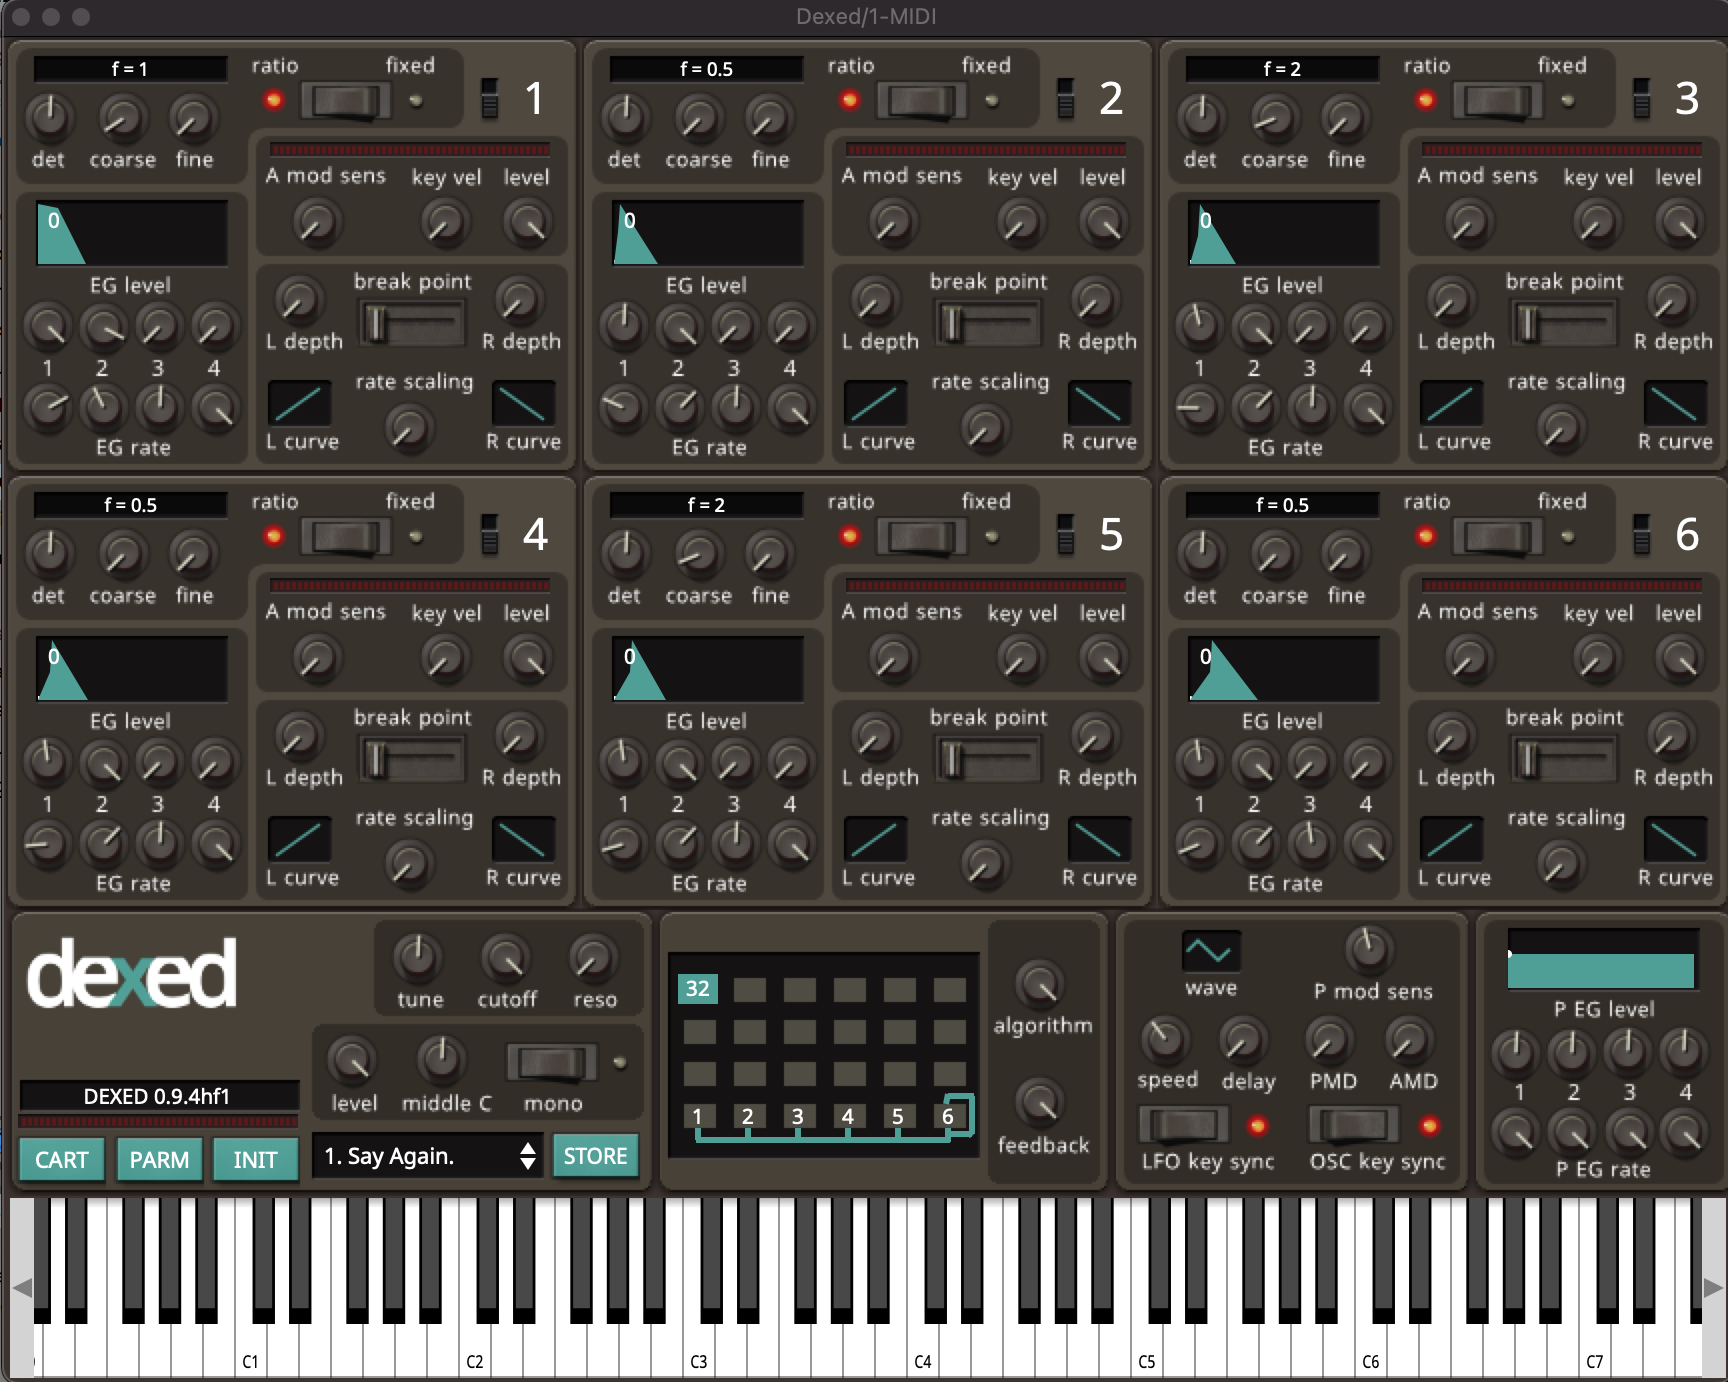
\includegraphics[width=0.75\textwidth]{figures/spiegelib/dexed.png}
    \caption{The Dexed synthesizer interface. Dexed is an open-source emulation of the Yamaha DX7 FM synthesizer and it was used in the experiments in this chapter/}
    \label{fig:dexed}
\end{figure}

\begin{figure}[ht]
    \centering
    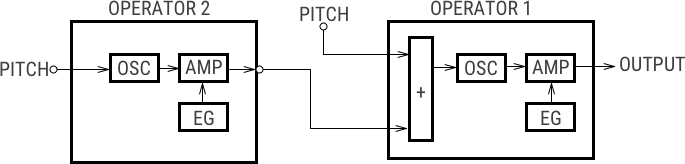
\includegraphics[width=0.9\textwidth]{figures/spiegelib/two_op_fm_block.png}
    \caption{Block diagram of a two operator FM synthesizer. Dexed has six independent operators that can be configured in various ways, however for the experiments conducted here only the first two operators were used and were setup in this configuration.}
    \label{fig:two_op_fm_block}
\end{figure}

\begin{figure}[ht]
    \centering
    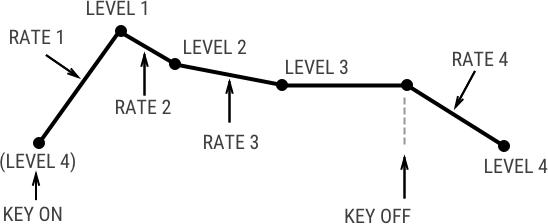
\includegraphics[width=0.75\textwidth]{figures/spiegelib/Yamaha DX7 Envelope.png}
    \caption{Diagram of an envelope generator in the Yamaha DX7 and Dexed. The envelope has five independent stages. During the first three stages the envelope moves linearly from level 4 to level 1, then to level 2, then to level 3. Each of these levels is controllable and the length of time taken to move to each level is also definable. This movement is triggered by a key-on event. Once the envelope has progressed to level 3 it stays at that level until a key-off event is received, at which point the envelope progresses back to level 4.}
    \label{fig:dx7_envelope}
\end{figure}

% \begin{table}[]
%     \centering
%     \begin{tabular}{c|c}
%          &  \\
%          & 
%     \end{tabular}
%     \caption{Caption}
%     \label{tab:my_label}
% \end{table}

\subsection{Dataset}
The \mintinline{python}{DatasetGenerator} class was then used to create datasets for deep learning training. All deep learning models, except for the CNN, used a 13-band MFCC calculated with a frame size of 2048 samples and a hop size of 1024 samples. The input of the CNN was the magnitude spectrum from a STFT, calculated using an FFT with 512 bins and a hop size of 256 samples. Using an instance of \mintinline{python}{DatasetGenerator}, 50,000 training examples and 10,000 validation examples were generated by randomly sampling the nine parameters from $Dexed$. Resulting feature vectors were normalized by removing the mean and scaling to unit variance using methods within the \mintinline{python}{FeatureBase} base class. Datasets and settings for normalization were then stored as NumPy files for later use.

\subsection{Estimation Techniques}
List out all the techniques used in the experiment.

\subsection{Models}
All deep learning models are defined in classes within \mintinline{python}{spiegelib} and all inherit from \mintinline{python}{TFEstimatorBase}. Three models derived from work by Yee-King et al. \cite{yee2018automatic} were used: 1) A simple multi-layer perceptron with three hidden layers, all with a ReLu activation, 2) a LSTM recurrent network with three layers and dense output, and 3) a LSTM++ networks which contains a single bidirectional LSTM node followed by a dense layer with an elu activation, six highway layers, and a dense output. One convolutional neural network (CNN) derived from work by Barkan et al. \cite{barkan2019inversynth} was also included: this network featured six layers of strided convolutions followed by a dropout layer and a dense output. Specific details of all these models is provided in appendx \ref{appendix:spiegelib_models}.

Models were trained using an $Adam$ optimizer \cite{kingma2014adam} with a learning rate of 0.001, batch sizes of 64, and used an early stopping callback which halted training if validation loss was stagnant for 10 epochs to prevent overfitting. Ideally the loss function would be computed directly on audio rendered from $Dexed$ using the predicted parameters, but that is challenging to implement, so the loss is computed on the parameter values which has been standard in previous work \cite{yee2018automatic, barkan2019inversynth}.

The loss function used was the RMS error between the target parameter values and the predicted parameter values, which is given by the following formula where $N$ is the number parameters, $y$ is the true parameter values, and $\hat{y}$ is the predicted parameter values:

\begin{equation}
    \ell(y, \hat{y}) = \sqrt{\frac{\sum_{i \in N}{(y_i - \hat{y_i})^2}}{N}} 
\end{equation}

Logging of training and validation progress was recorded using the \mintinline{python}{TFEpochLogger} class. Plots of training and validation accuracy and loss for the LSTM++ model are shown in figure \ref{fig:lstm_bi_train}. 

% TODO: add in some of the other loss plots (probably all of them) and remark on the differences betwee them.

Trained models are then saved for future use.

\begin{figure}[ht]
\begin{center}
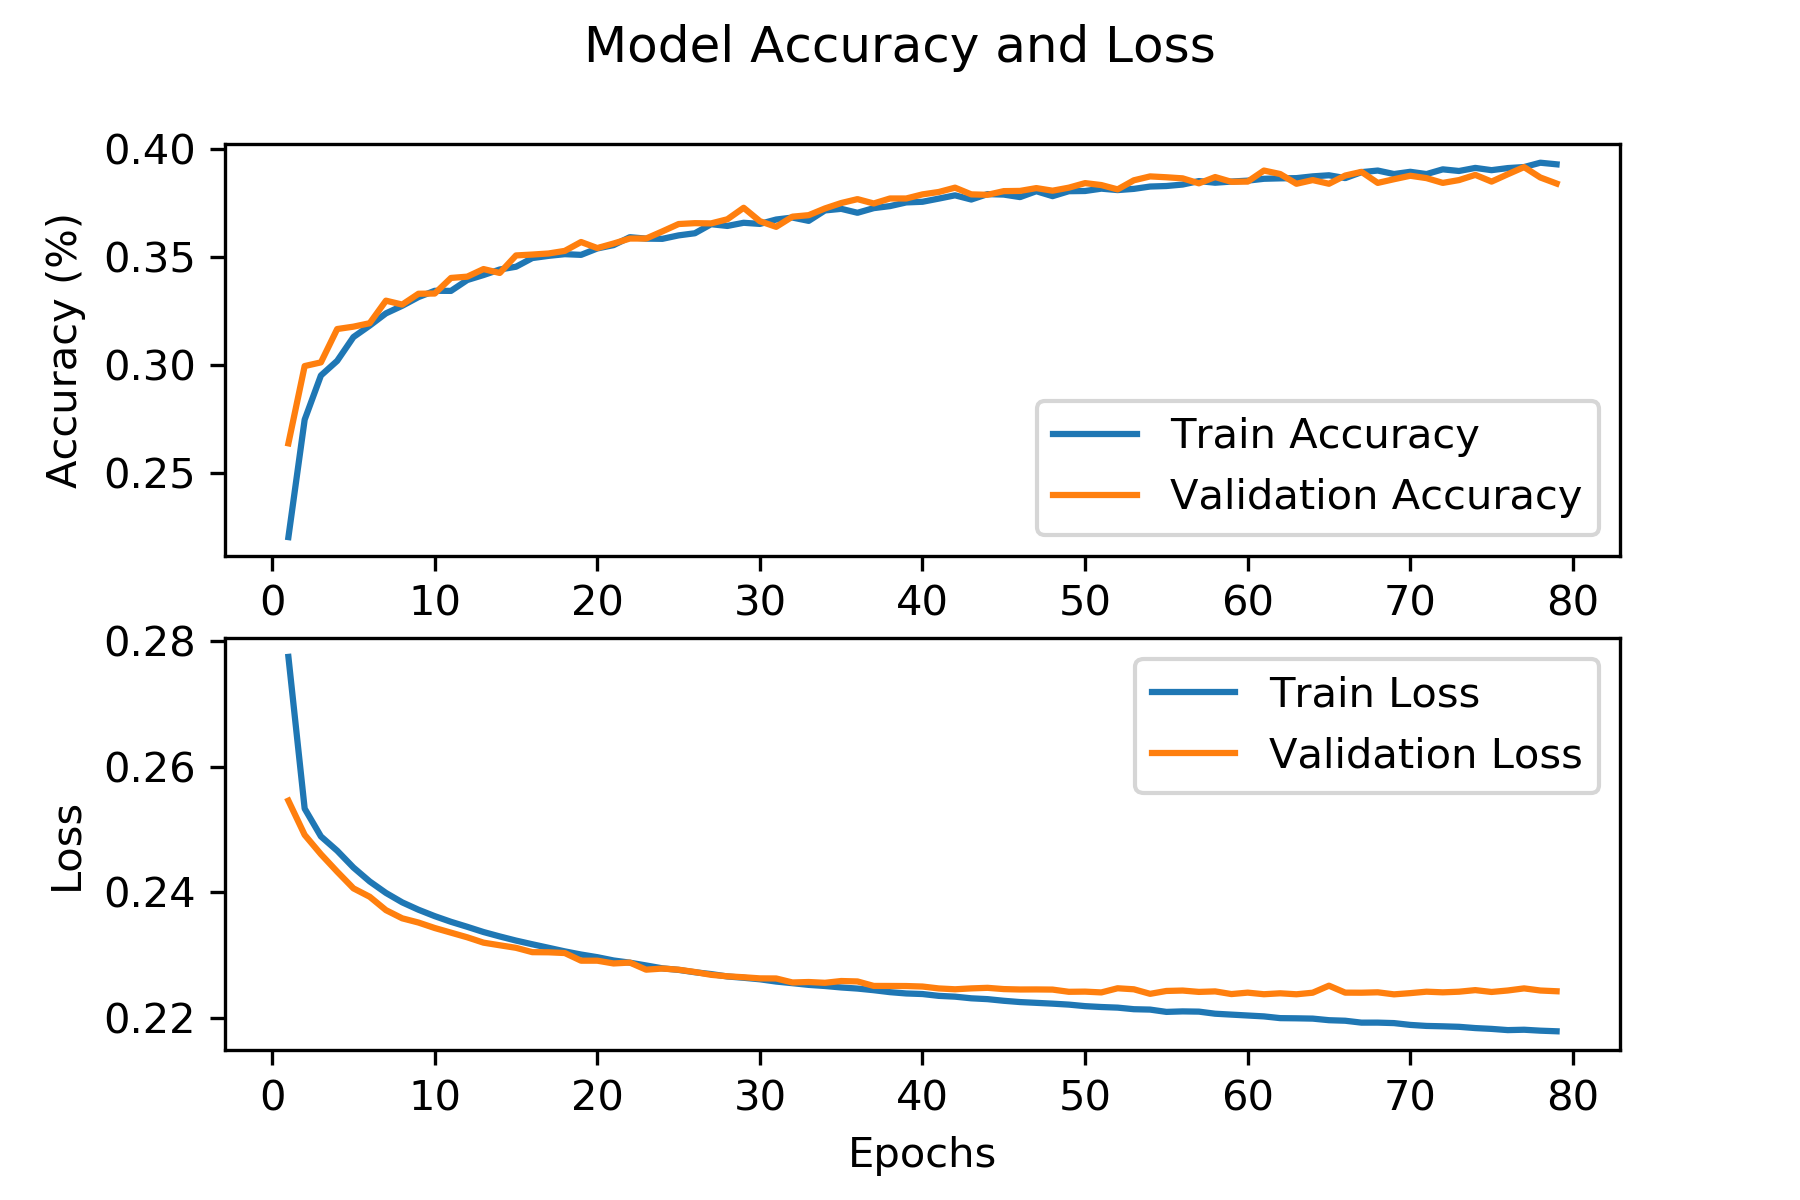
\includegraphics[width=0.75\columnwidth]{blstm_training.png}
\caption{Traing and validation accuracy and loss over epochs for LSTM++ model training.}
\label{fig:lstm_bi_train}
\end{center}
\end{figure}

\subsection{Genetic Algorithms}
Two different GAs were used: a basic single-objective GA and a multi-objective NSGA III. The multi-ojective GA was derived from work conducted by \cite{macret2012automatic} that used the algorithm to automatically tune the parameters of a Teenage Engineering OP-1\footnote{\url{https://teenage.engineering/products/op-1}} synthesizer. In the GAs the $fitness$ (which is equivalent to the loss in deep learning) is easily computed directly on the audio rendered from $Dexed$. In the case of the basic GA the $fitness$ is computed as the mean absolute error (MAE) between 13-band MFCCs from the target and the individual. Three different metrics were used for evaluating the $fitness$ of an individual for the NSGA-III algorithm, MAE between: 1) a 13-band MFCC, 2) magnitude spectrum from an FFT, and 3) five spectral features. MAE is given by the following formula, where $N$ is the number of features, $y$ is the target, and $\hat{y}$ is the predicted individual:

\begin{equation}
    \text{MAE} = \frac{\sum_{i \in N}{|y_i - \hat{y}_i|}}{N}
\end{equation}

Both genetic algorithms were run for 100 generations for each sound target. The basic GA and NSGA used population sizes of 300 and 100 individuals respectively. Figure \ref{fig:nsga_fitness} shows the minimum spectral error achieved by an individual during each iteration of the NSGA algorithm on one of the target sounds. The plot shows a period of rapid improvement during early iterations, with some short periods of stagnation, followed by longer periods where the algorithm is unable to find an individual that is an improvement over those in the current population.

% TODO: Add in the other population generation plots for each objective

\begin{figure}[ht]
\begin{center}
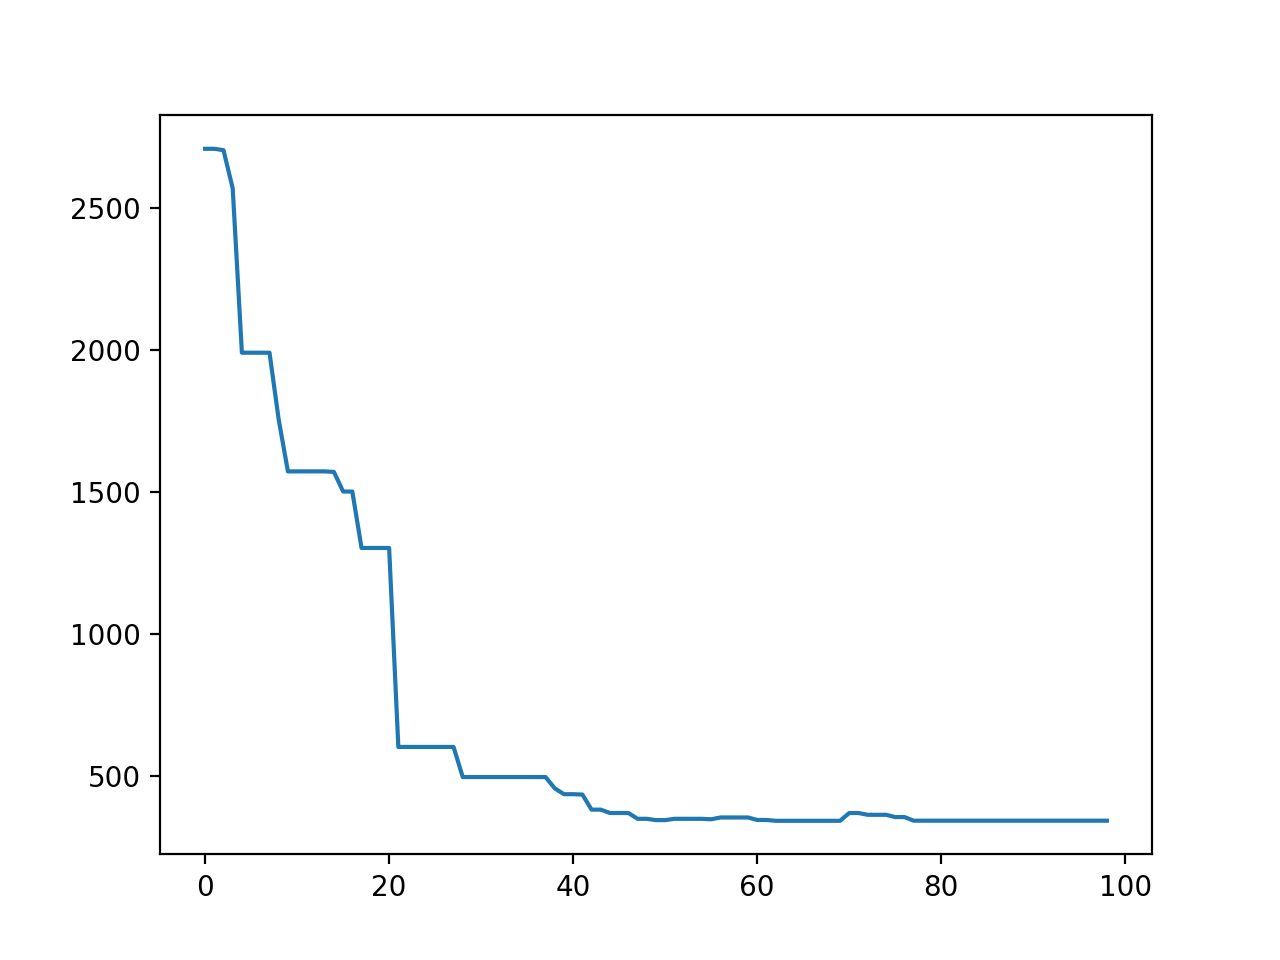
\includegraphics[width=0.7\columnwidth]{nsga_target_15_FFT.png}
\caption{Minimum FFT MAE in the population at each generation to target sound 15 for NSGA III estimator.}
\label{fig:nsga_fitness}
\end{center}
\end{figure}

\section{Evaluation}
To evaluate each of the techniques an evaluation dataset containing 25 random sounds generated using the same nine-parameter $Dexed$ configuration was used. Using the sounds generated using the same synthesizer configuration means that an error of zero is possible, which provides a stable baseline for comparing each of the methods. All estimators were run on each one of the 25 target sounds using the \mintinline{python}{SoundMatch} class. This resulted in a set of audio files generated from $Dexed$ using the estimated parameters from each estimator run on each of the 25 target sounds. All of the resulting sounds are available for listening online on the SpiegeLib docs page\footnote{\url{https://spiegelib.github.io/spiegelib/examples/fm_sound_match_pages/fm_sound_match_listen.html}}. Quantitative and qualitative evaluation was conducted on these sounds.

\subsection{Quantitative Evaluation}
Evaluation was conducted by comparing the predicted audio files to the target audio using MAE computed on MFCCs, which is the same method that was used during evaluation by Yee-King et al. \cite{yee2018automatic}. Results for mean absolute error (MAE) which have been summarized using mean, standard deviation, minimum, and maximum, are shown for each estimator in table \ref{tbl:sound_match_eval}. Both GAs performed better than the deep learning approaches with the NSGA III having the best overall score. For deep learning approaches, the LSTM++ model achieved the best mean score. 

% TODO informal listening based on MAE so I can comment on the results in terms of MAE

Histograms of the the MAE were also plotted for each estimator using the \mintinline{python}{plot_hist()} method in \mintinline{python}{EvaluationBase}. Histograms of the MAE for all predictions made by all estimators are shown in figure \ref{fig:group_hist}. These plots clearly show the NSGA III as the winner in terms of MFCC MAE; 24/25 of the predicted sounds have an MAE less than 2.5 (the smallest histogram bin), and the other sound is still less than 5. For the deep learning models, the LSTM++ performed the best overall, however the LSTM model produced more results that had a MAE less than 2.5. The MLP model performed the worst overall and the histogram shows a wide range of results, the MLP also produced a result with the worst individual score of 34.12. The CNN model performed only slightly better than the MLP and had no predictions with a score less than 2.5.

% TODO objective evaluation based on the parameter values?

\subsection{Qualitative Evaluation}
Spectrograms of one target sound and sound match predictions made by each of the estimators for that target are shown in figure \ref{fig:group_spect}. The selected example was one of the most challenging targets; both the GAs, the LSTM, and the MLP method received their worst individual score on it. The most clear difference between the spectrograms can be seen in the temporal evaluation of the harmonics, which is caused by the EG applied to the amplitude of the second operator. In the target the envelope slightly decreases over the course of the first half of the sound and then remains constant until the end.

% TODO finish off this section.

For this particular target, spectrograms reveal that while the frequency and distribution of the harmonics was relatively close for each estimation, all estimators except for the NSGA III struggled with matching the temporal envelope of the spectrum.

\begin{table}[t]
\centering
\caption{Results from sound matching evaluation}
\label{tbl:sound_match_eval}
\begin{threeparttable}
\begin{tabular}{l|cccc}
\toprule
$Method$ & $Mean$ & $SD$ & $Min$ & $Max$ \\
\midrule
$MLP$ & 8.55 & 6.77 & 1.92 & 34.12 \\
$CNN$ & 7.88 & 4.26 & 2.68 & 20.89 \\
$LSTM$ & 6.12 & 3.76 & 1.20 & 19.36 \\
$LSTM++$ & 4.91 & 6.50 & 2.12 & 21.51 \\
$GA$ & 2.25 & 2.58 & 0.70 & 11.17 \\
$NSGA III$ & \textbf{0.81} & \textbf{0.89} & \textbf{0.001} & \textbf{3.06} \\
\bottomrule
\end{tabular}
\begin{tablenotes}[para, flushleft]
\footnotesize
\item Values shown are calculated from the mean absolute error (MAE) calculated during MFCC evaluation. Smaller MAE values indicate more similar matches. The NSGA III estimator received the best scores, which are shown in bold font.
\end{tablenotes}
\end{threeparttable}
%\vspace{5mm}
\end{table}

\begin{figure}[t]
\begin{center}
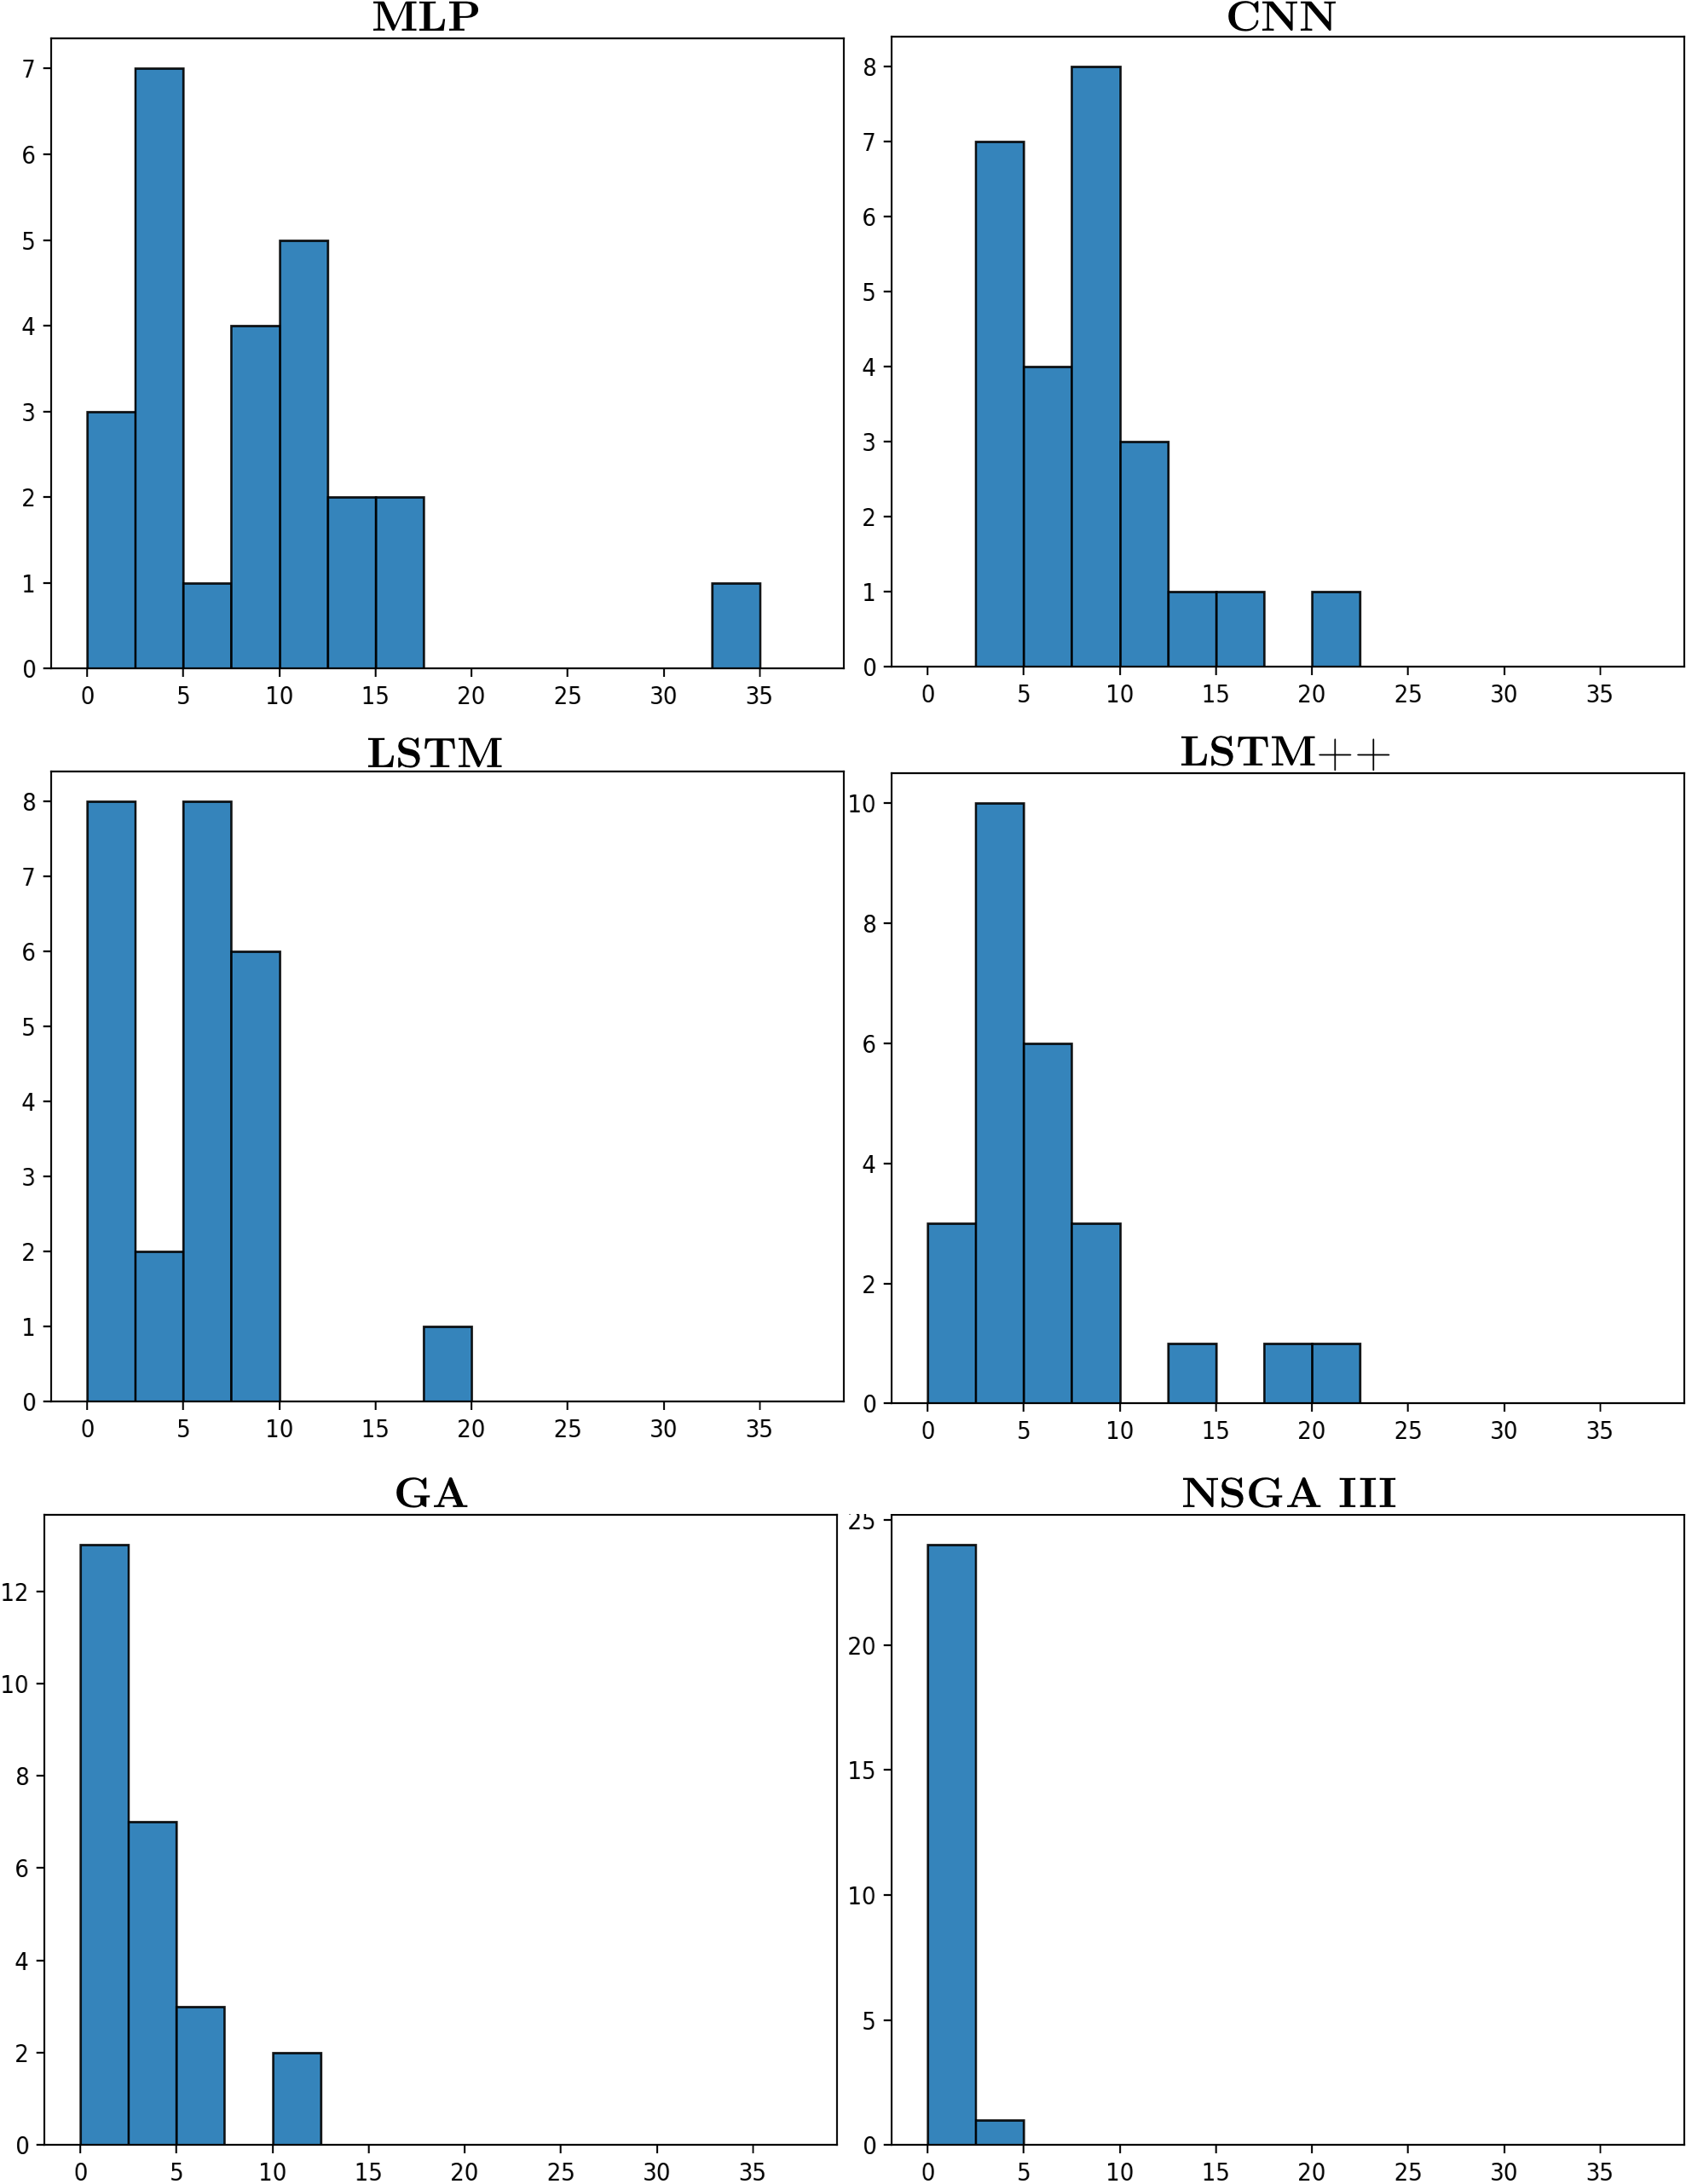
\includegraphics[width=0.75\textwidth]{hist_group_v3.png}
\caption{Histogram shows the MAE values resulting from MFCC evaluation run on a set of 25 sound targets for all estimators. Lower MAE values indicate a closer sound match.}
\label{fig:group_hist}
\end{center}
\end{figure}

\begin{figure}[t]
\begin{center}
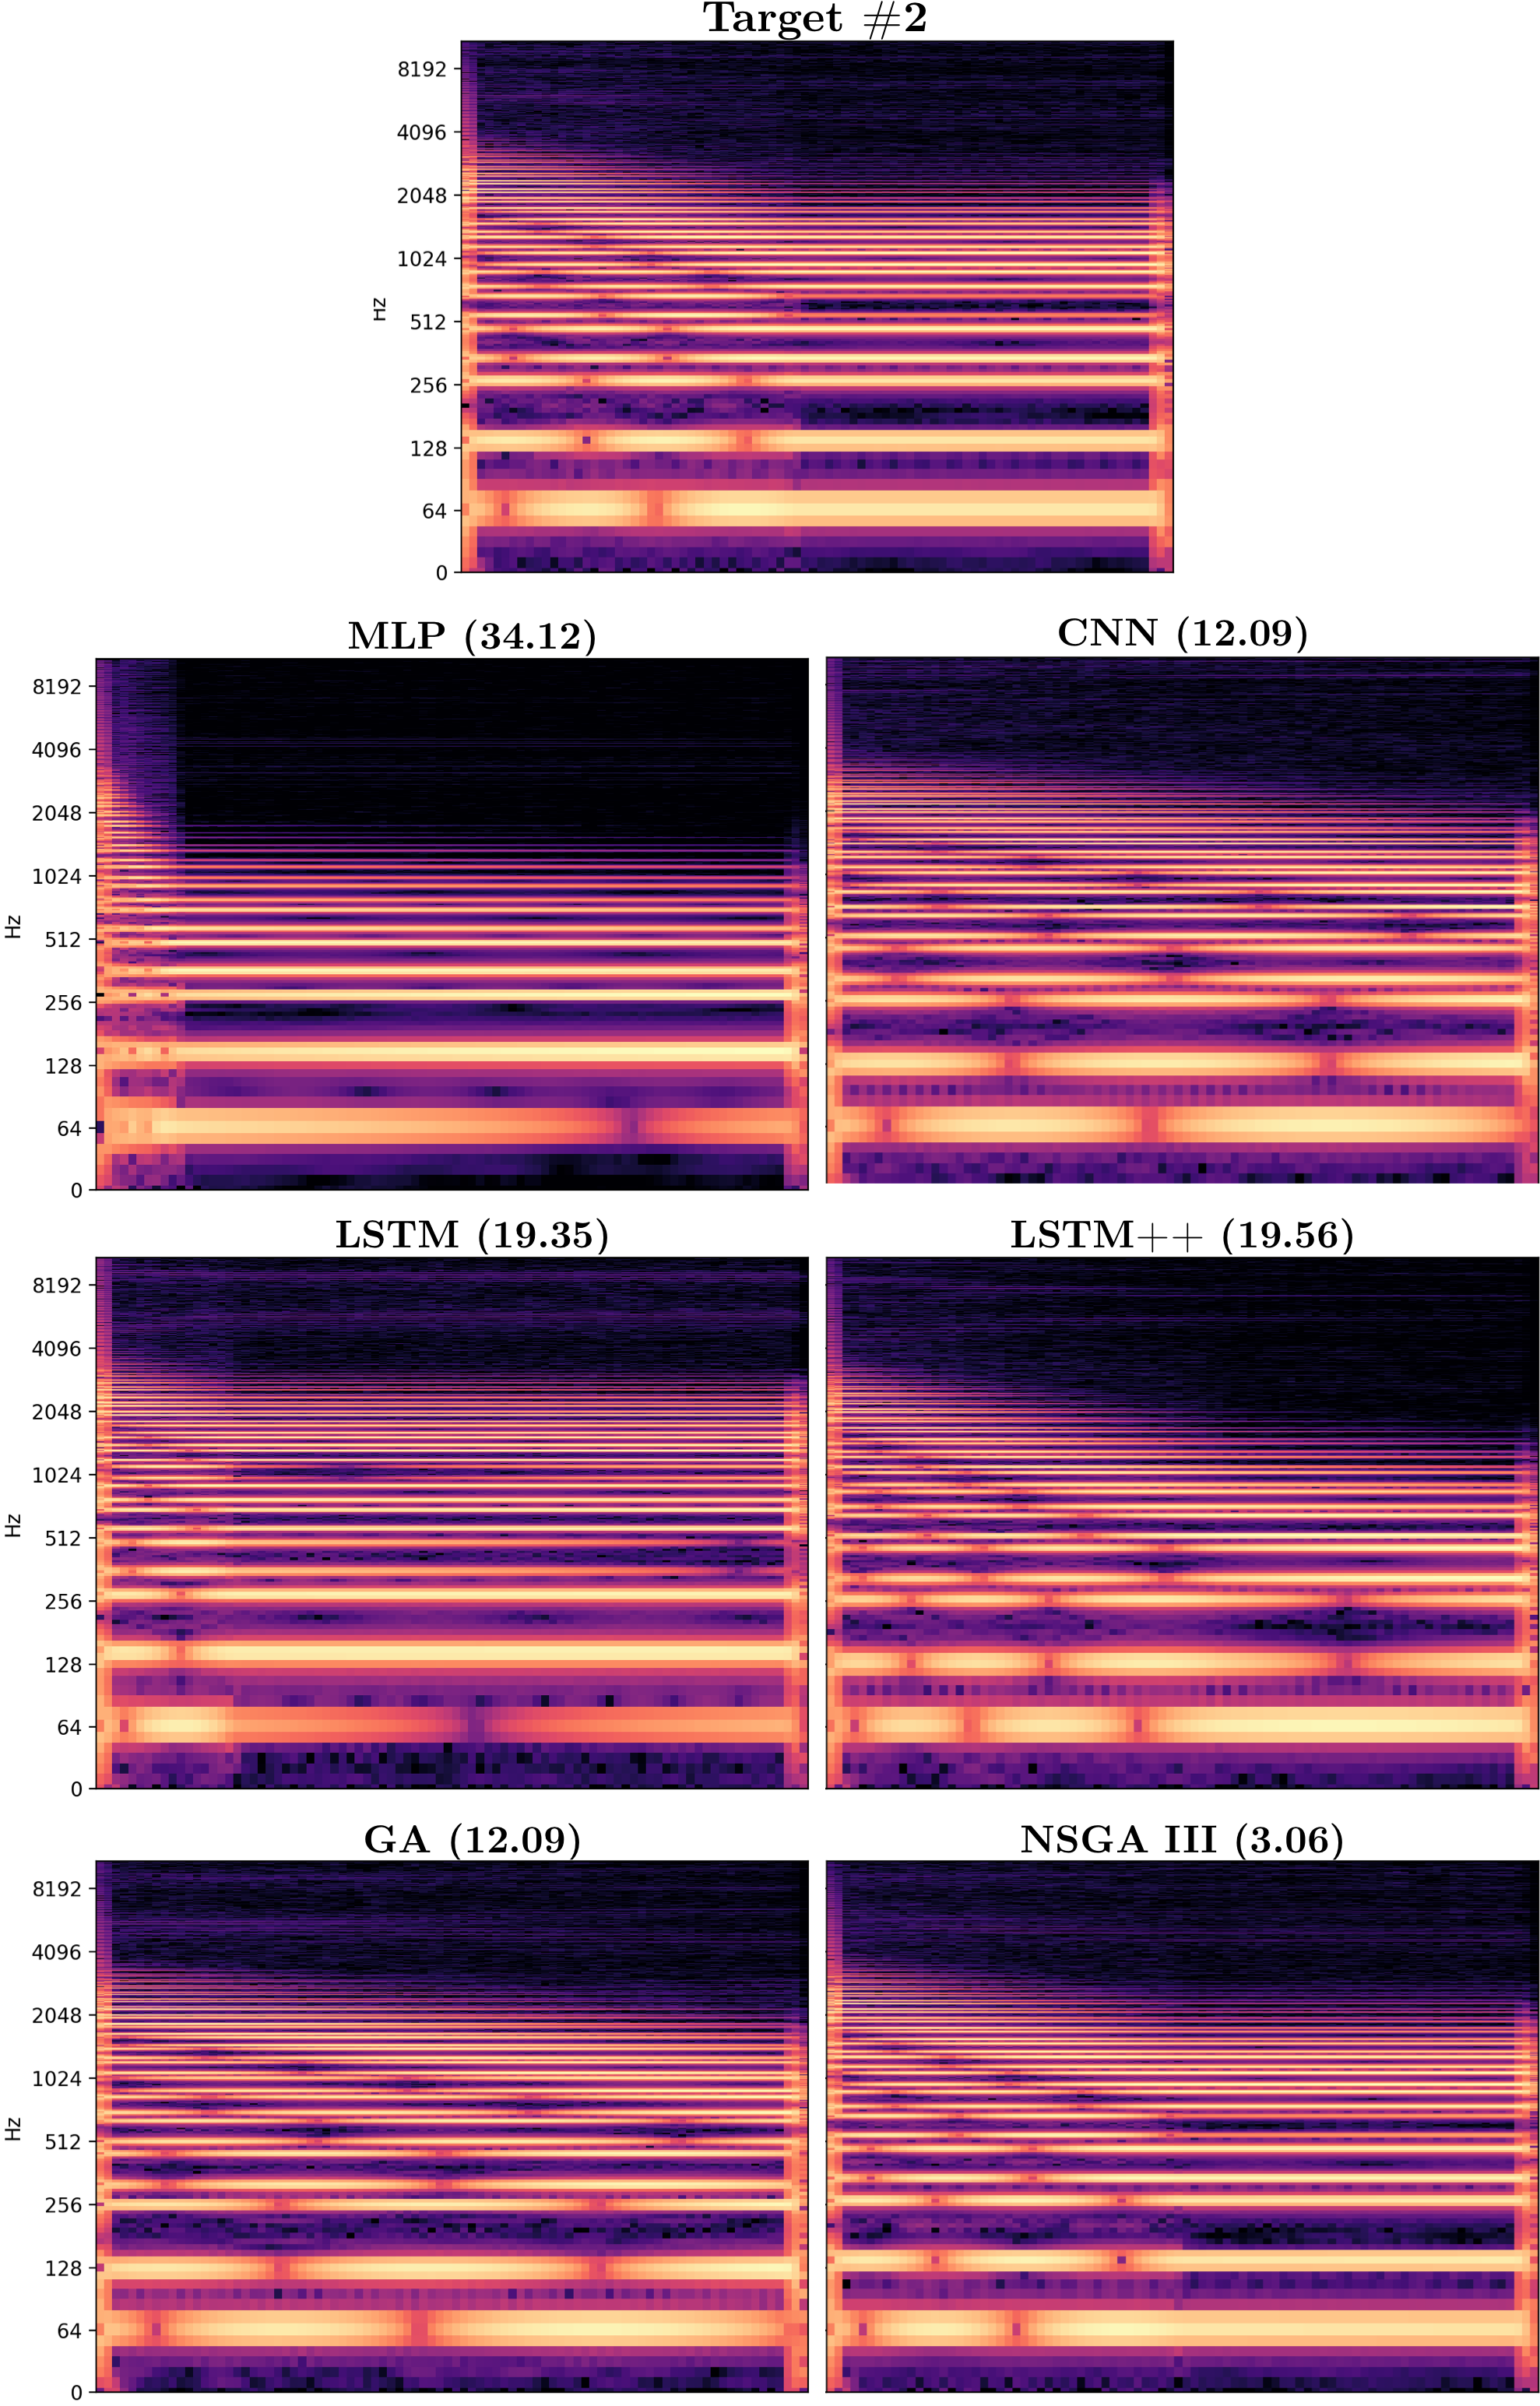
\includegraphics[width=0.75\textwidth]{spect_group_v1.png}
\caption{Spectrogram plots of a target sound and sound match predictions made by each estimator. The value next to the estimator name is the MAE value from MFCC evaluation for that prediction (lower MAE values indicate a closer match).}
\label{fig:group_spect}
\end{center}
\end{figure}

To evaluate to the resulting predictions the \mintinline{python}{MFCCEval} class was used, which calculates error and distance metrics on MFCCs of a target and prediction. Results for mean absolute error (MAE) which have been summarized using mean, standard deviation, minimum, and maximum, are shown for each estimator in table \ref{tbl:sound_match_eval}. Both GAs performed better than the deep learning approaches with the NSGA III having the best overall score. For deep learning approaches, the LSTM++ model achieved the best mean score. Histograms of the the MAE were also plotted for each estimator using the \mintinline{python}{plot_hist()} method in \mintinline{python}{EvaluationBase}. Histograms of the MAE for all predictions made by all estimators are shown in figure \ref{fig:group_hist}. Spectrograms of one target sound and sound match predictions made by each of the estimators for that target are shown in figure \ref{fig:group_spect}. For this particular target, spectrograms reveal that while the frequency and distribution of the harmonics was relatively close for each estimation, all estimators except for the NSGA III struggled with matching the temporal envelope of the spectrum.

% If we have time!!
%\subsection{Tunefish: Interactive Genetic}

\section{Future Work and Conclusion}
Development of \mintinline{python}{spiegelib} is ongoing and a number of expansions to the current library are planned. First, we would like to continue to expand the number of estimators available and plan on integrating the following: a hill climbing optimizer \cite{yee2018automatic}, a particle swarm optimizer \cite{heise2009automatic}, more 2D CNN configurations \cite{barkan2019inversynth}, a 1D CNN for raw audio input \cite{barkan2019inversynth}, and a generative approach \cite{esling2020flow}.  Second, we would like to expand on the type of interactions available such as automatic programming from vocal imitations \cite{mcartwright2014} and interactive methods. 
%Third, we would like to integrate more sophisticated subjective evaluation tools such as creating links to setup tests using the Web Audio Evaluation Tool \cite{waet2015}. Third, we would like to contribute to the $RenderMan$ library that is used in this work in order to extend support to Windows users and distribute the library via PyPI so the entire \mintinline{python}{spiegelib} library can be installed in one command. 
Finally, we would like to encourage developers and researchers from the automatic synthesizer programming community to contribute to \mintinline{python}{spiegelib}. Information on contributing is available online.\footnote{\url{https://spiegelib.github.io/spiegelib/contributing.html}} 

This work has introduced \mintinline{python}{spiegelib}, an open-source automatic synthesizer programming library. \mintinline{python}{spiegelib} is an object-oriented library that was designed with the goal of supporting development, collaboration, and reproducibility in the field. The library includes implementations of classes for conducting ASP research. These classes contain functionality for interacting with VST synthesizers, extracting audio features, creating datasets, estimating synthesizer parameters, and evaluating results. Six implementations of deep learning and evolutionary parameter estimation techniques based on previous work are included, with more planned. An example case of an automatic synthesizer sound matching study using the library was shown. This example case, along with the supporting code and data available online showcases how \mintinline{python}{spiegelib} can be used to support reproducible research.
